\section{Executable scalar algorithms and reproducible computations}
\label{sec:computation}

The fixed-dimensional algorithms above establish bit-complexity bounds; they
are not efficient general implementations of real quantifier elimination.
This section
gives executable specializations with a scalar leader for three distinct
tasks: certifying a proposed convex response path, constructing a complete
nonconvex response graph, and optimizing an upper problem over that graph.
An exact follower oracle at finitely many prices does not solve a continuous
leader problem.

\subsection{Convex quadratic paths and an aligned sweep}
\label{subsec:convex-implementation}
Consider the unique response on the unit box to
\begin{equation}\label{eq:implemented-convex}
 \min_{0\le z\le1}\ \tfrac12z\trans Qz+(c+Cx)\trans z,
 \qquad Q=D+UHU\trans\succ0,\quad x\in[L,R],
\end{equation}
where $x$ is scalar, all data are rational, $D$ is positive diagonal, $H$ is
symmetric, and the displayed decomposition is supplied. The implemented upper
problem minimizes
\begin{equation}\label{eq:implemented-upper}
 o_xx+o_z\trans z+o_{xx}x^2+x\,o_{xz}\trans z
 \quad\text{subject to}\quad a_jx+b_j\trans z\le h_j.
\end{equation}
Tariff maximization is represented by a negative $x$--response coefficient;
the nonconvex interface below maximizes revenue directly.

For a status assignment with free coordinates $F$ and upper coordinates $B$,
set $z_B=1$, set the remaining bound coordinates to zero, and solve
\[
 Q_{FF}z_F=-c_F-C_Fx-Q_{FB}\mathbf1.
\]
The solution is a rational affine function of $x$. Free-coordinate bounds and
bound-gradient signs give its exact closed validity interval; degenerate zero
gradients are allowed. The affine stationarity identities and the signs at the
two endpoints of the interval certify KKT throughout the interval, and positive
definiteness makes this the unique global response. This is the familiar
active-set mechanism of explicit parametric quadratic programming
\citep[Theorems 2 and 4]{BemporadEtAl2002}; here the certificate also verifies
coverage of the entire requested price interval.

No inverse of $H$ is required. For a right-hand side $v$, put
$S=U_F\trans D_F^{-1}U_F$ and solve
\[
 (I+SH)w=U_F\trans D_F^{-1}v,
 \qquad z_F=D_F^{-1}(v-U_FHw).
\]
The determinant identity
$\det Q_{FF}=\det D_F\det(I+SH)$ proves invertibility, even when $H$ is singular
or indefinite. For rank $k$, a pattern solve uses
$O(N(1+k^2)+k^3)$ rational arithmetic operations, excluding validation of the
supplied positive-definiteness assumption. The implementation checks that
assumption with small-rank sufficient tests and, when these do not apply, with
direct exact matrix tests.

\begin{proposition}[Certified and exhaustive convex paths]
\label{prop:convex-certified-path}
A finite collection of rational affine pieces for \eqref{eq:implemented-convex}
is a complete exact response path if every piece passes the preceding KKT test
and its closed intervals cover $[L,R]$. Enumerating all $3^N$ status assignments
always produces such a path. On any certified complete path,
\eqref{eq:implemented-upper} is solved exactly by rational arithmetic.
\end{proposition}
\begin{proof}
On a box, KKT is necessary and sufficient for a convex differentiable
objective. Every optimizer, including one at a degenerate boundary, has a
status assignment, so exhaustive enumeration covers every price. Conversely,
each certified piece contains only optimizers. Substitute its affine response
into each upper row and intersect the resulting intervals, retaining singleton
intersections. The upper objective becomes a rational quadratic. Its minimum is
attained at an endpoint or, when its quadratic coefficient is positive, at its
interior stationary point; compare these rational candidates. The least value
over the finite path solves the upper problem, or no piece is feasible and the
problem is certified infeasible.
\end{proof}

The generic implementation uses a numerical box-QP routine only to propose a
status assignment at a price in an uncovered gap. It tries several numerical
status tolerances, recomputes the proposed segment exactly, and verifies that
it contains the queried price; for small $N$ it can fall back to exhaustive
search. It returns a path only after exact KKT and coverage verification;
otherwise it raises a recovery or coverage error. Reaching the segment cap and
unsuccessful numerical proposals are explicit failure modes. No numerical
tolerance is used to declare global coverage; nevertheless, the procedure is not an unconditional
polynomial-time path-construction algorithm.

For the aligned rank-one case $Q=D+h uu\trans\succ0$ and $C=\gamma u$ with
$\gamma>0$, a simpler sweep is complete. Define
\[
 z_i(t)=\clip_{[0,1]}(-(c_i+u_it)/d_i),\qquad A(t)=u\trans z(t).
\]
Zero entries of $u$ give constant coordinates; each nonzero entry gives at
most two rational breakpoints. On a multiplier interval,
$A(t)=A_0+A_1t$, with $A_1=-\sum_{i\in F}u_i^2/d_i$. The relation
\begin{equation}\label{eq:convex-sweep-inversion}
 x=(t-hA(t))/\gamma,\qquad
 t=(\gamma x+hA_0)/(1-hA_1)
\end{equation}
is strictly increasing: every free principal matrix is positive definite,
so $1+h\sum_{i\in F}u_i^2/d_i>0$. This includes negative $h$ whenever the
whole Hessian is positive definite. The map tends to $\pm\infty$ on the
tails and therefore covers every price. Updating the affine coefficients at
each grouped breakpoint gives the complete response path. Maintaining the
weighted response sums in the objective and the $m$ upper rows takes
$O(N\log N+N(m+1))$ rational arithmetic operations, not bit operations;
only the selected response is reconstructed in all coordinates. Sorting and
clipped multiplier allocation are classical resource-allocation ingredients \citep{Kiwiel2008}; the implementation
combines them with exact upper-interval optimization. The sweep and the upper
solve are fused, so their timings are reported together.

\subsection{Complete nonconvex scalar compression}
\label{subsec:nonconvex-compression}
The second specialization allows an indefinite follower Hessian:
\begin{equation}\label{eq:nonconvex-implemented}
 f_x(z)=\sum_{i=1}^N\left(\tfrac12d_i z_i^2+c_i z_i\right)
       -\tfrac h2(u\trans z)^2+\gamma x u\trans z,
 \quad \ell\le z\le r,\quad x\in[L,R].
\end{equation}
Here $N\ge1$, all data are rational, $d_i>0$, $h\ge0$, $\gamma\ne0$, $\ell_i\le r_i$,
and $L\le R$. Signed and zero $u_i$, fixed coordinates, negative prices,
and either sign of $\gamma$ are allowed. The upper problem maximizes $xw$,
where $w=u\trans z$, subject to rational affine upper rows. Optimistic and
pessimistic selection follow Section~\ref{sec:foundations}, with maxima and
suprema in place of minima and infima.

Let $[w_-,w_+]$ be the image of the follower box under $u\trans z$, and define
\begin{equation}\label{eq:scalar-fiber-value}
 C(w)=\min\left\{\sum_i(\tfrac12d_i z_i^2+c_i z_i):
                  \ell\le z\le r,\ u\trans z=w\right\},
 \qquad \psi(w)=C(w)-\tfrac h2w^2.
\end{equation}
The fiber problem is strictly convex even when \eqref{eq:nonconvex-implemented}
is nonconvex, so its minimizer $z(w)$ is unique. Every global follower optimum
is the minimizer on its own fiber; otherwise its objective could be decreased
without changing the aggregate terms. Thus the original global problem is
exactly $\min_{w\in[w_-,w_+]}\{\psi(w)+\gamma xw\}$, and $z(w)$ recovers the
actual responses.

\begin{lemma}[Rational fiber pieces]\label{lem:scalar-fiber-pieces}
If $w_-<w_+$, the interval has at most $2N-1$ nondegenerate pieces on which
$z(w)$ is rational affine and $\psi(w)$ is rational quadratic. They and their
endpoints can be constructed in polynomial bit complexity. If $w_-=w_+$,
there is one constant aggregate and one unique fiber response.
\end{lemma}
\begin{proof}
For a multiplier $\lambda$, strict convexity gives
\[
 z_i(\lambda)=\clip_{[\ell_i,r_i]}((\lambda u_i-c_i)/d_i).
\]
For $u_i=0$ this means the constant clipped unconstrained minimizer. Ignore
fixed coordinates when forming events. Sort the at most $2N$ numbers
$(d_i\ell_i+c_i)/u_i$ and $(d_ir_i+c_i)/u_i$ for $u_i\ne0$.
On each interval between consecutive events, $z=a+b\lambda$ and
$w=w_0+S\lambda$, with $S=\sum_{i\in F}u_i^2/d_i\ge0$.
If $S>0$, invert to obtain $z(w)$. If $S=0$, the interval maps to a single
aggregate already supplied by its adjacent pieces; the two infinite tails
likewise supply only endpoints. By continuity of clipping, the union
covers $[w_-,w_+]$. The fiber KKT equations and strict convexity show that the
recovered response is the unique fiber optimum, also at shared endpoints.
Substituting it into \eqref{eq:scalar-fiber-value} gives each quadratic.
If all aggregates are equal, the box constraints fix the coordinates with
nonzero $u_i$, and the others minimize independently. Rational sums, products,
sorting and inversions give polynomial bit bounds. Storing every length-$N$
affine response explicitly takes at most quadratic, rather than linear, storage.
\end{proof}

Write a piece as $\psi(w)=Aw^2+Bw+D$ on $[a,b]$. Its complete list of minimizer
candidates under the price tilt is:
\begin{enumerate}
\item its endpoints, available at every price;
\item if $A>0$, the stationary point $w=-(B+\gamma x)/(2A)$ on the rational
price interval where it lies in $[a,b]$;
\item if $A=0$, the whole interval $[a,b]$ at $x=-B/\gamma$.
\end{enumerate}
A piece with $A<0$ contributes only endpoints. Stationary candidates have
quadratic value functions in $x$; endpoint candidates have affine ones.
All candidates are feasible, so globality is decided by comparing their
\emph{original} values, not by stationarity alone.

\begin{theorem}[Complete scalar atlas and upper optimization]
\label{thm:nonconvex-atlas}
For \eqref{eq:nonconvex-implemented}, a finite exact response description and
the upper tariff problem under both selection conventions can be computed
in polynomial bit complexity.
The description consists of rational affine responses on open price intervals
with algebraic endpoints of degree at most two, together with all isolated
responses and all flat fiber intervals at individual prices. The algorithm
decides upper feasibility, computes the supremum and its attainment, and
returns an attaining response when one exists. Each reported optimizer or
limiting pair, together with its value, belongs to one field of degree at most
two; different atlas cuts may lie in different quadratic fields. Optimistic
feasibility implies attainment; pessimistic feasibility need not.
\end{theorem}
\begin{proof}
Form all candidate domain endpoints, all flat-piece prices, and every real
crossing of two candidate value polynomials in their common domain. Include
$L,R$ and discard prices outside $[L,R]$. There are $O(N^2)$ cuts, each rational
or quadratic algebraic. On each open interval between cuts, a rational sample
determines the valid candidates and every comparison sign. Keep all global
winners. At every cut, compare all valid candidates anew, adding a flat interval
exactly when its value equals the global minimum. This proves completeness,
including isolated ties and lower-dimensional price strata.

On an open interval, two winning value polynomials must agree identically.
Their derivatives equal $\gamma w(x)$, for endpoint and stationary
candidates alike. Since $\gamma\ne0$, they describe the same aggregate, and
uniqueness of the fiber minimizer gives the same original response. Distinct
optimal responses can therefore coexist only at the recorded individual prices.

For an open interval, substitute the affine response into the upper rows.
Their intersection is an interval, possibly empty or a singleton inside the
original open interval. Maximize its quadratic revenue by comparing endpoint
limits and any interior stationary point with negative quadratic coefficient.
Also retain an interior rational sample to recognize attainment of a constant
value. Flag an endpoint as attained only if it belongs to the original open
price interval; the upper inequalities themselves are closed.

At a recorded price, each optimal response component is $z(w)$ on a singleton
or a closed fiber interval. Optimistically, intersect each component with all
upper rows and maximize the linear function $xw$ on what remains.
Pessimistically, require every upper row at both endpoints of every component,
then take the least $xw$ over all those endpoints. These endpoint tests are
exact because $z(w)$ is affine on a fiber piece. Comparing the finite list of
values and one-sided limits gives the supremum. Prefer an attained candidate
when its value ties a limit; if none attains the best value, return the limiting
price and aggregate with an explicit nonattainment flag. The optimistic graph
is closed in a compact box, which gives a separate proof of optimistic
attainment. This closedness argument does not apply to the pessimistic problem.

The all-pair construction has polynomially many branches, cuts and comparisons,
and all rational coefficient lengths are polynomial in the input. Quadratic
root isolation and comparison, including comparisons between different
quadratic fields, have polynomial bit complexity. A rational sample between
distinct quadratic cuts can be found by dyadic refinement with polynomial bit
length. Upper stationary points and nontrivial row boundaries on open pieces
are rational, and so are flat-piece prices; every remaining endpoint output
lies in the field of its one quadratic price. Thus no reported optimizer or
value requires the compositum of all switch fields.
\end{proof}

The executable compressed implementation inserts candidates one at a time into
the current lower envelope. On each existing envelope interval it splits at the
new candidate's validity boundaries and at its crossings with the current
winner, then compares at rational interior samples. It keeps the resulting
envelope and a separate set of contact prices, including tangencies. Finally it
compares \emph{all} original candidates at the retained contacts and flat
prices. This shorter list suffices. Consider a final global tie at the moment
the later of the two tied branches was inserted. No branch existing then could
have had smaller value there. The tie was therefore at a current boundary, a
new domain boundary, or a crossing with a current winner, unless the value
polynomials coincided. In that last case their derivatives give the same
response, so no distinct contact is missed. An isolated-domain candidate also
contributes its domain endpoint. Consequently the incremental construction
preserves every final global contact. Conservative bounds are $O(N^2)$ retained
cuts and $O(N^3)$ interval processing steps. The implementation retains full
response vectors and uses symbolic arithmetic, so these counts do not predict
its practical running time.

\subsection{Convex-envelope values and original contacts}
\label{subsec:contacts}
Extend $\psi$ by $+\infty$ outside $[w_-,w_+]$. Its conjugate gives
\begin{equation}\label{eq:contact-conjugacy}
 v(x)=-\psi^*(-\gamma x)
     =\min_w\{\psi^{**}(w)+\gamma xw\}.
\end{equation}
To verify the second equality, put $m=\min_w(\psi(w)+\gamma xw)$. The affine
function $m-\gamma xw$ minorizes $\psi$ and hence lies below its closed convex
envelope $\psi^{**}$. The minimum on the right is therefore at least $m$ and,
because $\psi^{**}\le\psi$, at most $m$. The original minimizers are exactly
\begin{equation}\label{eq:actual-contact}
 \{w:\ \psi^{**}(w)+\gamma xw=v(x),\quad \psi(w)=\psi^{**}(w)\}.
\end{equation}
The second condition is essential for upper feasibility and tie-breaking.
Convex envelopes of piecewise quadratic functions and their conjugates have
established algorithms: Gardiner and Lucet
\citep[Propositions 3.1 and 4.3]{GardinerLucet2010} give quadratic and linear
arithmetic-time constructions, and Moehle et al.~\citep[Section 6.3 and
Appendix B]{MoehleEtAl2023} give a further constructive account. We do not
claim to improve these envelope bounds. Our direct candidate proof supplies
the original contact sets and rational-bit guarantees needed here, without a
tangent formula from an external implementation.

\begin{example}[False choices from convexification]\label{ex:false-contacts}
Take $N=1$, $d=u=1$, $c=-1$, $h=3$, $\gamma=1$, $z\in[0,1]$,
and $x\in[1,3]$. Then $\psi(z)=-z^2-z$ has convex envelope $-2z$.
The actual response is $1$ for $x<2$, $0$ for $x>2$, and $\{0,1\}$ at
$x=2$. The convexified response at $2$ is the entire interval $[0,1]$.
Consequently upper rows requiring $z=1/2$ are infeasible for the original
bilevel problem, although convexification admits revenue $1$. Mixing the
two original optima cannot repair this discrepancy. Without those rows,
the optimistic maximum is $2$, attained at $(2,1)$, whereas the pessimistic
supremum is $2$ and is not attained.
\end{example}

\begin{example}[Capacity at an interior jump]\label{ex:capacity-jump}
Let $d=(1,1)$, $c=(-1,-1/2)$, $u=(1,1)$, $h=3/5$, $\gamma=1$,
$z\in[0,1]^2$, $x\in[0,1]$, and impose the upper row $w\le1$. The fiber
formula is
\[
\psi(w)=\begin{cases}
 w^2/5-w,&0\le w\le1/2,\\
 -w^2/20-3w/4-1/16,&1/2\le w\le3/2,\\
 w^2/5-3w/2+1/2,&3/2\le w\le2.
\end{cases}
\]
At $x_*=17/20$, the only tilted minima are $w=3/8$ and $13/8$, both of
value $-9/320$, giving responses $(3/8,0)$ and $(1,5/8)$. The middle piece
is strictly concave, and its endpoints have value $-1/40$, so it supplies no
further minimizer. For $x<x_*$, comparison with the larger contact shows that
every optimal $w$ is at least $13/8>1$: a smaller $w$ has nonnegative
excess value at $x_*$ and gains strictly less from the negative price change.
For $x>x_*$, comparison with the smaller contact forces $w\le3/8$, and
minimization on the low piece gives $w=(5/2)(1-x)$, whose revenue decreases
on $[x_*,1]$. At $x_*$ only the smaller contact satisfies the capacity row.
Thus the optimistic maximum is $51/160$, attained at $x_*$, while the
pessimistic supremum is the same number and is not attained. This is a failure
of universal upper feasibility at a tie, not a failure to compute the nominal
global follower value.
\end{example}

\begin{figure}[t]
\centering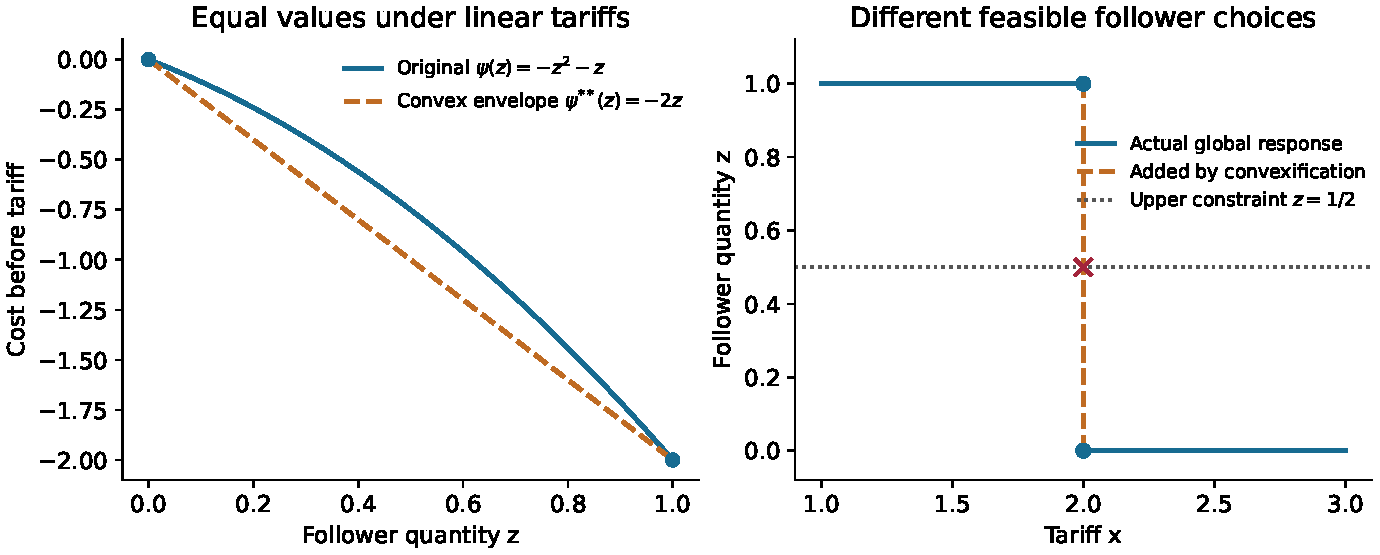
\includegraphics[width=.96\linewidth]{figures/contacts.pdf}
\caption{Example~\ref{ex:false-contacts}. Left: the original aggregate cost and
its convex envelope. Right: original responses retain two contacts at the
switch; the additional vertical segment admitted by convexification consists
of false follower choices.}
\label{fig:contacts}
\end{figure}

Local stationarity is also insufficient: on $[0,1]$,
$f(z)=z/4-z^2/2$ has a strict one-sided local minimum at $0$, of value $0$,
but its global minimum is at $1$, of value $-1/4$. Both points satisfy box KKT.
The examples and the atlas construction therefore treat global selection
explicitly.

\subsection{An independent original-coordinate baseline}
\label{subsec:full-task-baseline}
To compare complete bilevel tasks, we implement a second solver directly in
original coordinates. Enumerating stationary faces of a box quadratic is
classical; see, for example, the discussion in \cite{HladikCernyRada2021}.
The baseline extends this validation to the full price interval and both upper
selection conventions. It shares rational instance data with the compressed
method, but no fiber allocation, envelope construction or upper-optimization
code. It requires that \emph{every principal minor} of
$Q=\diag(d)-huu\trans$ be nonzero: it checks all $2^N-1$ nonempty minors
and rejects an unsupported instance before solving. This restriction excludes
flat follower directions; the compressed method has no such restriction.

\begin{proposition}[Completeness of the original-coordinate baseline]
\label{prop:original-face-baseline}
Under the stated nonzero-principal-minor restriction, enumerating original
stationary box faces, comparing their original objective values over the
whole price interval, and retaining all ties yields the complete response
graph of \eqref{eq:nonconvex-implemented}. The upper tariff problem under both selection conventions, including
attainment, are then solved exactly. Enumeration is exponential in $N$.
\end{proposition}
\begin{proof}
Take any global minimizer and its minimal box face. On its free coordinates
$F$, first-order stationarity holds and the second-order necessary condition
makes $Q_{FF}$ positive semidefinite; its nonzero determinant then makes
it positive definite. Hence this optimizer appears in an enumerated face with
\[
 z_F(x)=-Q_{FF}^{-1}(c_F+\gamma u_Fx+Q_{FB}z_B).
\]
Here $B$ contains both lower and upper fixed coordinates. The baseline
solves this dense original-coordinate system, rejects free faces that are not
positive definite, and intersects the free bounds and bound-gradient signs to
get an exact rational validity interval. A coordinate whose lower and upper
bounds coincide needs no gradient sign. Each retained candidate is feasible,
and every global optimum is retained. Comparing their \emph{original} quadratic
values therefore gives exactly all global optima, regardless of nonglobal KKT
points.

Substitution into $\tfrac12z\trans Qz+(c+\gamma xu)\trans z$ gives a rational
quadratic in $x$. Form all validity endpoints and all pairwise value crossings
on overlaps, including crossings above the global envelope. Exact comparison
on open cells and separately at their endpoints retains all ties. The
nonzero-minor condition rules out a missing continuum: any minimizer in a
positive-dimensional minimal face is the unique stationary point just solved.
Equal winning value polynomials on an open cell have equal derivatives
$\gamma u\trans z$ and hence equal aggregate responses; strict fiber convexity
then makes the entire responses equal.

The baseline independently clips each open response cell with the upper rows
and compares quadratic revenue at endpoints, stationary points and interior
samples, tracking whether each endpoint belongs to the cell. At a cut,
optimistic selection compares all upper-feasible global responses; pessimistic
selection requires all global responses to satisfy the rows and takes their
least revenue. This finite decomposition proves the upper result, including
nonattainment. There are at most $3^N$ faces and quadratically many pair
comparisons in that number; each solve and comparison uses exact rational or
quadratic algebraic arithmetic.
\end{proof}

An earlier independent oracle enumerates original stationary faces at a
single requested price. It may skip singular free faces and still find the
global \emph{value}: a stationary positive-semidefinite singular face has a
null direction along which the quadratic is constant, and moving to the
boundary reduces the face until it is nonsingular or a vertex. This does not
recover a whole flat minimizer set or optimize over all prices; the checked
restriction of the original-coordinate baseline is what makes it a
complete-response and complete-upper-task comparison.

\subsection{Computational protocol and findings}\label{subsec:computations}
All fresh runs use the rational data and deterministic generators in the
accompanying code and data archive, on Linux with an Intel Xeon w5-2565X,
Python 3.13.11, SymPy 1.14.0, NumPy 2.5.1 and SciPy 1.18.0. Each reported
fresh timing is the median of three serial fresh-process runs; all individual
times, wrapper warnings and solver output are retained. OpenBLAS, OpenMP, MKL
and NumExpr were set to one thread, and the SciPy MILP calls also passed
\texttt{threads=1} to HiGHS. Each process starts with the SymPy cache cleared,
and paired methods alternate their order between repetitions to control
shared-cache effects. The machine was shared; we claim no hardware isolation or
statistical speed guarantee. All 60 recorded workers completed within an
external 90-second limit, so no timed-out run is omitted.

The correctness tests compare both global upper outcomes on eight adversarial
and ten seeded small random instances. They compare the entire response sets at
every cut of the baseline's independently constructed face partition and at
an interior sample of each of its cells. For each attained output of \emph{both} methods, they
check bounds, $w=u\trans z$, revenue, every upper row, and the original
follower cost against all valid original-coordinate faces at the returned
price. These returned prices include upper-row boundaries and stationary
revenue points, not just follower switches. Pessimistic witnesses also undergo universal
feasibility and least-revenue checks. Separate tests of the compressed method
cover flat intervals, fixed boxes and singleton aggregates.

Further diagnostics exercise exact convex path certification, forced
numerical-proposal failures, corrupted certificates and missing coverage;
nonconvex original-face value comparisons on signed and fixed-coordinate
instances; and incremental-envelope contacts against a full pairwise partition.
The convex checks include negative rank-one coefficients with positive-definite
total Hessian, nearly singular rational data, and data outside floating-point
range. These finite checks, whose counts are recorded by test family, test
the implementation contracts and specified failure modes; they are not a
formal verification of the general theorems.

\paragraph{The same continuous leader task.}
The heterogeneous family draws $d_i$ uniformly from
$\{8,\ldots,16\}/8$, $u_i$ from $\{4,\ldots,8\}/4$, and $-c_i$ from
$\{4,\ldots,24\}/8$, in that order, with seed $17+N$. It has the unit box,
$x\in[0,5]$, $h=(7/5)/(\sum_i u_i^2/d_i)$, and upper capacity
$u\trans z\le\tfrac12\sum_i u_i$. Its Hessian is indefinite: diagonal
congruence gives $I-hvv\trans$ with $v\trans v=\sum_i u_i^2/d_i$, which has one
negative eigenvalue. Both methods construct the whole response graph and solve the upper problem
under \emph{both} selection conventions with the same upper rows.
Table~\ref{tab:full-task} also includes Example~\ref{ex:capacity-jump}.
Every exact value and attainment flag agrees between the methods and across
repetitions. By total and wall time, the original-coordinate baseline is
faster on the jump and $N=4$ instances, and the compressed method is faster
on the heterogeneous $N=2,6$ instances.
Neither method is uniformly faster, even on these small complete tasks.
The exponential baseline was deliberately limited to $N\le6$, where it checks
at most 63 principal minors and 729 statuses. Larger instances were not
attempted with it, so none is reported as a timeout.

\begin{table}[t]
\centering\small
\caption{Fresh full-task comparisons, seconds (three-run medians).
Faces denotes the original-coordinate baseline; its build includes input
parsing and principal-minor validation. Opt. and pess. solve the upper problem
under the two selection conventions after construction.
Total includes solver input validation, construction and both upper solves;
wall also includes process startup, imports and input-file reading.
Each column is an independently computed median.}
\label{tab:full-task}
\begin{tabular}{llrrrrr}\toprule
$N$ & Method & Build & Opt. & Pess. & Total & Wall\\\midrule
2 (jump) & Compressed & 0.1322 & 0.0102 & 0.0057 & 0.1473 & 0.4348 \\
2 (jump) & Faces & 0.0034 & 0.0007 & 0.0004 & 0.0046 & 0.3018 \\
2 & Compressed & 0.0597 & 0.0014 & 0.0010 & 0.0623 & 0.3541 \\
2 & Faces & 0.1112 & 0.0005 & 0.0004 & 0.1121 & 0.4082 \\
4 & Compressed & 0.6924 & 0.0973 & 0.0665 & 0.8490 & 1.1772 \\
4 & Faces & 0.3334 & 0.2220 & 0.1637 & 0.7074 & 1.0160 \\
6 & Compressed & 0.7014 & 0.2130 & 0.1479 & 1.0605 & 1.3984 \\
6 & Faces & 0.6413 & 0.4266 & 0.3480 & 1.4041 & 1.7100 \\
\bottomrule
\end{tabular}
\end{table}

\paragraph{Symbolic cost and population structure.}
Profiling the unmodified scalar implementation on the $N=12$ heterogeneous
family showed that repeated symbolic cancellation in sign tests dominated the
cost: 5.74 of 9.88 profiled seconds (including instrumentation; not benchmark
times) across the build and one unconstrained upper solve. The copy
distributed with this paper (the \emph{paper copy}) makes two local changes:
it decides the sign of an already
rational expression directly, and it samples the rational midpoint of two
rational interval endpoints. The full exact algebraic fallback and the
candidate, envelope and contact logic are unchanged; the fallback still uses a
rational sample between unrelated quadratic cuts, avoiding unnecessary
output-field extensions.

In ordinary (unprofiled) fresh runs on the same constrained $N=12$ task,
build times were $3.150,2.929,3.107$ seconds for the unmodified
implementation and $2.748,2.679,2.708$ seconds for the paper copy; median
totals including both upper solves were $4.055$ and $3.605$ seconds,
respectively.
This modest improvement supports the two local changes but does not remove the
symbolic cost of heterogeneous events. Table~\ref{tab:scalar-scaling} reports
the remaining fresh scalar runs.

The two-type family has $N=2m$: $m$ copies of $(d,c,u)=(1,-1,1)$ and $m$
copies of $(1,-1/2,1)$, with $h=3/(5m)$, $x\in[0,1]$ and capacity $w\le m$.
Its Hessian is indefinite since $h\sum_i u_i^2/d_i=6/5$.
Uniqueness of the local fiber allocation makes coordinates within each type
equal. Dividing costs and aggregate by $m$ reduces the response problem exactly
to Example~\ref{ex:capacity-jump}. Therefore the optimistic optimum is
$51m/160$ at price $17/20$ and aggregate $3m/8$, while the pessimistic
supremum is the same and is not attained. There are three fiber pieces and seven
atlas points for every $m$. The $N=1000$ run thus tests repeated types, whereas
$N=48$ has 66 fiber pieces; their timings measure different structural regimes.

\begin{table}[t]
\centering\small
\caption{Fresh compressed scalar runs, seconds (three-run medians).
The last two upper columns concern the same capacity row. Total includes input
validation, build and both upper solves; process wall times and all repetitions
are in the data archive.}
\label{tab:scalar-scaling}
\begin{tabular}{lrrrrrr}\toprule
$N$ & Fiber pieces & Atlas points & Build & Opt. & Pess. & Total\\\midrule
12 & 21 & 45 & 2.7076 & 0.4769 & 0.4346 & 3.6053 \\
24 & 38 & 79 & 3.9774 & 0.8773 & 0.7808 & 5.6096 \\
48 & 66 & 135 & 13.6697 & 2.7917 & 2.8244 & 19.2916 \\
20 (two types) & 3 & 7 & 0.1365 & 0.0413 & 0.0331 & 0.2039 \\
200 (two types) & 3 & 7 & 0.1415 & 0.2125 & 0.2828 & 0.6275 \\
1000 (two types) & 3 & 7 & 0.2388 & 1.2650 & 1.6078 & 3.1009 \\
\bottomrule
\end{tabular}
\end{table}

The separate convex tariff family uses $u_i=1$, $h=1/(10N)$,
$d_i\in\{5,\ldots,20\}/10$, $-c_i\in\{1000,\ldots,25000\}/10000$,
$x\in[0,3]$, a service floor $\sum_i z_i\ge N/5$, and seeds $50001+N$.
The fused aligned sweep and upper solve had fresh median times of
$0.014$, $0.117$ and $1.100$ seconds for $N=100,1000,10000$, respectively;
input generation and validation added $0.0005$, $0.0032$ and $0.0336$ seconds.
Every returned response passed exact KKT and service-floor checks. These
synthetic convex results do not measure the nonconvex atlas or a general
large-scale bilevel model.

Earlier archived runs used different cache and repetition protocols, so
their differences from fresh timings are not controlled speedup estimates.
The older all-pair compressed implementation, a different comparator from the
original-coordinate baseline, kept 274 atlas points for $N=12$, compared with
45 after incremental envelope insertion; its recorded build medians were
$15.882$ and $3.079$ seconds. Archived timings were $18.699$ seconds for
construction and $2.922$ for one upper solve at heterogeneous $N=48$, $0.255$
and $1.261$ seconds at two-type $N=1000$ (three fiber pieces, seven atlas
points), and $1.047$ seconds for the convex $N=10000$ fused sweep. The earlier
generic convex-path runs retain their exact certificates and small dense-KKT
MILP comparisons; they support the certificate interface but do not guarantee
completeness of numerical proposals on arbitrary inputs.

\paragraph{Dense screening: a negative timing result.}\label{para:screening-results}
The exact screening prototype implements certified dense screening, in the
scalar-cell specialization of
Section~\ref{sec:robust-screening}. The identity surrogate has a diagonal
response cover; the true dense Hessian is a rational symmetric perturbation
with verified strict diagonal dominance. Screening fixes certified statuses,
and exact original KKT recovery enumerates the ambiguous ones. The bound
$M3^t$ counts recovery LPs only; dense inversion, cover construction and
certification are additional real computational costs.

The independent numerical comparator uses two binary variables $l_i,u_i$ per
coordinate and $g=Qz+c+Cx$, imposing
\[
 z_i+l_i\le1,\quad z_i-u_i\ge0,\quad l_i+u_i\le1,
 \qquad -M_i u_i\le g_i\le M_i l_i,
\]
with $0\le z_i\le1$ and
$M_i=1+|c_i|+|C_i|\max(|L|,|R|)+\sum_j|Q_{ij}|$.
If both binaries vanish, $g_i=0$; if $l_i=1$ or $u_i=1$, the corresponding
bound and gradient sign hold. Conversely, every box KKT point admits such
binaries, including zero-gradient bounds. By positive definiteness this is an
exact reformulation in real arithmetic. Its SciPy--HiGHS solve is numerical,
with a 30-second limit and requested relative MIP gap zero; numerical primal
and dual reports are not rational optimality certificates.

\begin{table}[t]
\centering\small
\caption{Screening versus dense KKT MILP, seconds. Archived entries are single
runs; fresh entries are three-run medians. Exact preprocessing includes input
generation and surrogate cover; exact total also includes final rational
verification. MILP preprocessing includes input generation and formulation.
Tighter-tolerance follow-ups are excluded from the default-solve columns.}
\label{tab:screening-negative}
\begin{tabular}{llrrrrrr}\toprule
 & &\multicolumn{3}{c}{Exact screening}&\multicolumn{3}{c}{Numerical MILP}\\
Source&$N$&Preprocess&Solve&Total&Preprocess&Solve&Total\\\midrule
Archived & 8 & 0.0034 & 0.0984 & 0.1023 & 0.0023 & 0.0243 & 0.0265 \\
Archived & 12 & 0.0141 & 0.2962 & 0.3112 & 0.0045 & 0.0382 & 0.0427 \\
Archived & 20 & 0.0142 & 0.9332 & 0.9509 & 0.0078 & 0.1560 & 0.1638 \\
Archived & 40 & 0.0334 & 17.5689 & 17.6121 & 0.0256 & 0.4041 & 0.4297 \\
Fresh & 8 & 0.0046 & 0.1273 & 0.1335 & 0.0025 & 0.0180 & 0.0203 \\
Fresh & 20 & 0.0200 & 0.9056 & 0.9293 & 0.0084 & 0.1624 & 0.1699 \\
\bottomrule
\end{tabular}
\end{table}

The exact prototype was slower on all four archived instances, and the fresh
$N=8,20$ repetitions confirm this after including preprocessing
(Table~\ref{tab:screening-negative}). Their maximum ambiguity is two, with
105 and 285 completed cell/status assignments. The archived $N=40$ case has
maximum ambiguity four and 2304 completed assignments; rational recovery alone
took $15.29$ of $17.57$ solver seconds.

The default $N=8$ MILP reports optimality and zero gap but an objective
$3.3703\cdot10^{-7}$ below the exact value
$4810519997/235205877942$, with a modeled-row violation of approximately
$3.5387\cdot10^{-7}$. This discrepancy occurs in the archived run and in
all fresh repetitions. With primal and MIP feasibility tolerances
$10^{-9}$, the objective agrees within $3.82\cdot10^{-17}$ and the maximum
row violation is $1.11\cdot10^{-16}$. At $N=20$, agreement is within $1.34\cdot10^{-15}$. The returned
exact screening solutions satisfy all rows and dense KKT equations rationally;
their global guarantee rests on the screening theorem, not on checking a
returned point alone.

The supplement preserves the rational instances, generator seeds, input
hashes, software and machine metadata, individual timings and exact diagnostic
logs. The experiments establish reproducible behavior for the stated scalar
subclasses only. They do not implement the general quantifier-elimination
algorithms and give no evidence of superiority on industrial instances or
arbitrary heterogeneous follower populations.
